\documentclass{article}
\usepackage{url}
\usepackage{graphicx}
\usepackage{listings}

\def\toolname{HOG}
\author{William Blum\\ Oxford University Computing Laboratory}


\title{A tool for constructing structures generated by higher-order recursion schemes and collapsible pushdown automata}



\begin{document}
\maketitle
\begin{abstract}
This is a brief documentation for \toolname (temporary name), a tool that allows one to explore the
infinite tree generated by higher-order recursion schemes and collapsible pushdown automata.
 The executable files and sources in OCaml/F\# can be downloaded from \url{http://web.comlab.ox.ac.uk/oucl/work/william.blum/}.

\end{abstract}

\section{Background}
The reader is referred to De Miranda's thesis \cite{demirandathesis} for an introduction to higher-order recursion schemes. Higher-order collapsible pushdown automata (CPDA for short) were introduced by Hague et.~al \cite{hmos-lics08}. The equivalence between the two devices is shown in the paper.
The algorithm that is used by \toolname\ to convert a recursion scheme to a CPDA is also described in
it.

\section{Features}

\toolname\ allows you to load a recursion scheme and observe the infinite tree generated by it.
It can also convert it to an equivalent CPDA of the same order whose infinite tree can in turn be explored. You also have the possibility to convert the recursion scheme to an order-$n$ PDA. The latter conversion is correct (in the sense that the same tree is generated) provided that the original recursion scheme satisfies the ``safety restriction'' \cite{KNU02}. (The proof of correctness will be written down soon).

The current version does not allow you to load your own CPDA as the parser has not been implemented yet. Consequently you can only create CPDAs by converting an equivalent recursion scheme.


\section{Defining a recursion scheme}
\label{sec:defrecscheme}
A recursion scheme is defined in a file with the .rs extension.
The syntax is self-explanatory. As an example, consider the higher-order recursion scheme formally defined by
$\langle \Sigma, \mathcal{N}, \mathcal{R}, S \rangle $
where $\Sigma = \{f:o\rightarrow o\rightarrow o, a:o \}$, $\mathcal{N} = \{
S: o, F: ((o \rightarrow o \rightarrow o)\rightarrow o\rightarrow o) \rightarrow o, H: ((o \rightarrow o \rightarrow o)\rightarrow o\rightarrow o) \rightarrow o \rightarrow o \rightarrow o, I: o \rightarrow o \rightarrow o \rightarrow o,
    G: (o \rightarrow o \rightarrow o)\rightarrow o\rightarrow o \}$ and

\[\begin{array}{rll}
   S & \rightarrow & F\, G \\
    F\, \psi & \rightarrow &\psi\, (H\, \psi)\, a \\
    H\, \psi\, x\, y & \rightarrow & \psi\, (I\, x)\, y \\
    I\, x\, u\, v & \rightarrow & x \\
    G\, \phi\, z & \rightarrow &f\, (\phi\, (\phi\, z\, a)\,a)\,a
\end{array}\]

The syntax for defining this recursion scheme in a .rs file is as follows:

\begin{lstlisting}
// Commentary
name { "This is an example of tree-generating recursion scheme." }
validator { none } // ignore this
terminals {
    f:o->o->o;
    a:o;
}
nonterminals {
    S: o ;
    F: ((o -> o -> o)->o->o) -> o;
    H: ((o -> o -> o)->o->o) -> o -> o -> o;
    I: o -> o -> o -> o;
    G: (o -> o -> o)->o->o;
}
rules {
    S = F G;
    F psi = psi (H psi) a;
    H psi x y = psi (I x) y;
    I x u v = x;
    G phi z = f (phi (phi z a)a)a;
}
\end{lstlisting}

Note that the first rule must be the one corresponding to the start symbol $S$.

\section{Usage}

If you start the program with arguments, it will try to open the file passed as a parameter. Otherwise
you can open a recursion scheme from the File$\backslash$Open menu.

\subsection{Recursion scheme}

Once a recursion scheme is opened, a window appears containing a description of the recursion scheme on the right and the value tree on the left. Of course, since the value tree is potentially infinite, it cannot be represented entirely, therefore it is presented to the user in a lazy way: At the beginning, only the root of the tree is shown containing the start symbol $S$. You can expand a branch of the tree by double-clicking on the corresponding node. When doing this, the expression contained in the node is evaluated using the OI-strategy (the head-redex is reduced by performing substitution) and new nodes are created for each terminal occurring in head position in the new expression.

\subsubsection{Computation graph}

If you click on the button ``Computation graph'' it will open up a new window containing the computation graph of the recursion scheme (obtained by computing the $\eta$-long normal form \cite{OngLics2006}).
Terminals are represented by rectangular nodes.
Non-terminals are shown in yellow, variables in dark green. In white
are the abstraction and application nodes. An example is given in Figure \ref{fig:compgraph}.

\begin{figure}[htbp]
  \begin{center}
  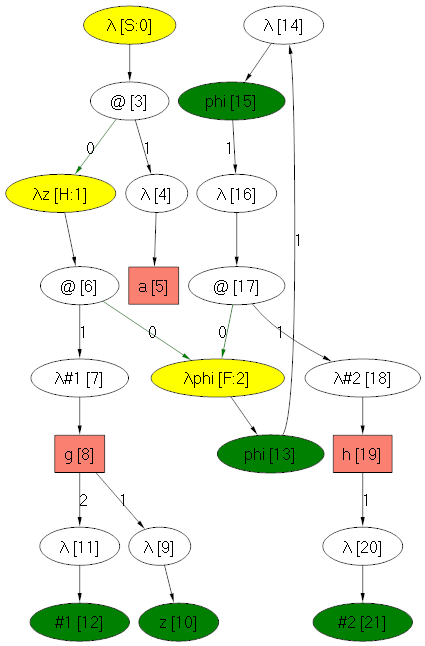
\includegraphics[width=10cm]{compgraph}
  \end{center}
  \caption{Computation graph generated from an order $2$-recursion scheme}\label{fig:compgraph}
\end{figure}


\subsubsection{Conversion to CPDA/PDA}

You can create the equivalent $n$-CPDA or $n$-PDA (provided that the recursion scheme is safe) by clicking on the appropriate button. This will open up a new window which allows you to explore
the value-tree generated by the CPDA (see section \ref{sec:cpda}).



\subsection{CPDA}
\label{sec:cpda}
The CPDA window is designed similarly to the recursion scheme window. The value tree is shown on the left
 and the description of the CPDA on the right.

\subsection{CPDA representation}
The transition function of the CPDA is given by a list of instructions.
A configuration of the CPDA is given by an instruction number together with an order $n$ stack.

\subsubsection{The CPDA code (the transition function)}
As mentioned before, the transition function of the CPDA is encoded with a list of instructions also
called the CPDA code. This code is shown on the right in the CPDA window.
 Each line of the CPDA code is made of three parts: the line number, an optional label and an instruction. There are four kinds of instructions: stack instructions, the node emitting instruction, branching instructions and debugging instructions. Except for branching instructions, the CPDA executes the code in a linear way:
 after performing an instruction it moves on to the following one.
 In the initial configuration, the CPDA is positioned on the first line of the CPDA code.

The stack instructions are:
\begin{description}
  \item[{\tt PUSH1 a (j,k)}] push the element {\tt a} on the top 1-stack an associates the link $(j,k)$ to it. This encoding means that the link points to a prefix stack obtained by performing an order-$j$ pop $k$ consecutive times.
  \item[{\tt PUSHn}] performs an order $n$ push on the stack (duplicates the top $n-1$-stack).
  \item[{\tt POPn}] performs an order $n$ pop on the stack (pop the top $n-1$-stack).
  \item[{\tt COLLAPSE}] collapses the stack to the prefix stack pointed to by the top element in the stack. In other words it executes $k$ times the execution {\tt POPj} where {\tt (j,k)} is the encoding of the link associated to the top element.

  \item[{\tt REPEAT n TIMES ins}] repeats the instruction {\tt ins} $n$ times where $n$ is a constant. The behaviour is unspecified if {\tt ins} is a branching instruction.
\end{description}

For the purpose of creating trees, there is an instruction that permits the CPDA to
create nodes:
\begin{description}
  \item[$\mathtt{EMIT\ f\ LAB_1 \ldots LAB_k}$] emits the terminal $f$ of type $o^k \rightarrow o$.
   The CPDA is then spawn into $k$ other CPDA's, one for each parameter of the terminal $f$.
   The $i's$ spawn CPDA will be started at instruction $\mathtt{LAB_i}$ for $i \in \{1..k\}$.
\end{description}

The branching instructions are:
\begin{description}
  \item[{\tt GOTO lab}] jumps to the label {\tt lab}.
  \item[$\mathtt{CASTOP0\ e_0->lab_0 ... e_k->lab_k}$] performs a test case on the element
  at the top of the stack. If the top element is equal to $\mathtt{e_i}$ for some $i \in \{0..k\}$
  then the CPDA jumps to the label $\mathtt{lab_k}$. Otherwise it moves on to the following instruction.
\end{description}

There are also instructions used for debugging the code of a CPDA:
\begin{description}
  \item[{\tt FAILWITH msg}] raises an exception with the message {\tt msg}.
  \item[{\tt ASSERT msg}] asserts that the condition described by the message {\tt msg} is verified. If the test fails then an exception is raised.
\end{description}

\subsubsection{Example}

This is an excerpt of the definition of the CPDA obtained by converting the recursion scheme given in section \ref{sec:defrecscheme}:

\begin{lstlisting}[breaklines=true]
Order: 2

Terminals:
h:o -> o
g:o -> o -> o
a:o

Stack alphabet: 0 1 2 3 4 5 6 7 8 9 10 11 12 13 14 15 16 17 18 19 20 21

Code:
 0                   PUSH1 0 (0,0)
 1 start          :  CASETOP0 0->NODE0 1->NODE1 2->NODE2 3->NODE3 4->NODE4 5->NODE5 6->NODE6 7->NODE7 8->NODE8 9->NODE9 10->NODE10 11->NODE11 12->NODE12 13->NODE13 14->NODE14 15->NODE15 16->NODE16 17->NODE17 18->NODE18 19->NODE19 20->NODE20 21->NODE21

 2 NODE0          :  PUSH1 3 (1,1)
 3                   GOTO start
 4 NODE1          :  PUSH1 6 (1,1)
 5                   GOTO start
 6 NODE2          :  PUSH1 13 (1,1)
 7                   GOTO start
 8 NODE3          :  PUSH1 1 (1,1)
 9                   GOTO start
10 NODE4          :  PUSH1 5 (1,1)
11                   GOTO start
12 NODE5          :  EMIT a // after this instruction the machine halts.
13 NODE6          :  PUSH1 2 (1,1)
14                   GOTO start
15 NODE7          :  PUSH1 8 (1,1)
16                   GOTO start
17 NODE8          :  EMIT g NODE8_1,NODE8_2
18 NODE8_1        :  PUSH1 9 (0,0)
19                   GOTO start
20 NODE8_2        :  PUSH1 11 (0,0)
21                   GOTO start
22 NODE9          :  PUSH1 10 (1,1)
23                   GOTO start
24 NODE10         :  REPEAT 5 TIMES POP1
25                   COLLAPSE
26                   CASETOP0 3->NODE10_3
27                   FAILWITH "Unexpected top 0-element!"
28 NODE10_3       :  PUSH1 4 (3,1)
29                   GOTO start
...
\end{lstlisting}

\subsection{Exploring the value tree by executing the CPDA code}

Each node of the (lazy) value tree corresponds to a configuration of the CPDA.
Nodes are labelled either by an instruction number or by a terminal.
When selecting a node, the content of the stack in the corresponding configuration
is shown in the textbox situated at the bottom of the right-hand side of the window.

At the beginning, the root node is labeled with the instruction number $0$ which corresponds to the first
instruction of the CPDA code. When double-clicking on a node, the corresponding CPDA instruction is executed. The corresponding stack is updated accordingly and the node label is updated to the next instruction to be executed. This process can be repeated until an {\tt EMIT} instruction is executed.

When a terminal $f:o^k\rightarrow o$ is emitted with the instruction
$\mathtt{EMIT\ f\ LAB_1 \ldots LAB_k}$, a node labelled $f$ is created in the value tree and $k$ children nodes are attached to it. Each child corresponds to a newly spawn CPDA with the same stack
and such that the $i$th child's starts at the instruction labelled with $\mathtt{LAB_i}$.

Terminal nodes represent the actual nodes of the value-tree and as such cannot be expanded further.

\bibliographystyle{plain}
\bibliography{../bib/dphil-all}
\end{document}
